% Created 2018-05-15 Tue 09:56
\documentclass[a4paper,11pt]{report}
                % input
                \usepackage[utf8]{luainputenc}
                \usepackage{fontspec}
                \usepackage{unicode-math}
                \usepackage[novoc]{arabluatex}
                \newfontfamily\arabicfont[Script=Arabic]{Scheherazade}
                \newcommand{\arbt}[1]{{\Large{\arb{#1}}}} %{\arbt{...}}
                \newcommand{\arbT}[1]{{\LARGE\arb{#1}}} %\arbT{...}
                % layout
                \usepackage{layout}
                \usepackage{setspace} %package pour les interlignes
                \usepackage{multicol}
                \setlength{\columnsep}{40pt}
                \usepackage{xcolor} % package pour les couleurs
                % headers ...
                \usepackage{fancyhdr} % header etc
                \usepackage{fancybox} %package pour les encadrements supp
                \pagestyle{fancy} % Use en-tetes et des pieds de page personnaliser grâce fancyhdr
                \usepackage[Glenn]{fncychap}
                \fancyhead[L, R, C]{} % définition en-tête
                \fancyfoot[L, R]{} % définition pied de page
                \fancyfoot[C]{\thepage}
           		\renewcommand{\headrulewidth}{0pt} % ligne haut out
	        	\renewcommand{\footrulewidth}{0pt} % ligne bas out
                % others
                \usepackage{float}
                \usepackage{array, makecell} %pour les tableaux et makecell pour les cellules
                \usepackage{multirow} %pr tableau
                \newcolumntype{P}[1]{>{\centering\arraybackslash}m{#1}} %P{taille}
                % maths
                \usepackage{amsmath, amsthm} %package pour les maths
                \usepackage{lettrine}
                \usepackage{marvosym} %package de symbole
                % others
                \usepackage{wrapfig} % pour les capsules in text
                %defaut emacs packages
                \usepackage{fixltx2e}
                \usepackage{graphicx}
                \usepackage{longtable}
                \usepackage{float}
                \usepackage{wrapfig}
                \usepackage{rotating}
                \usepackage[normalem]{ulem}
                \usepackage{textcomp}
                \usepackage{wasysym}
                \usepackage{hyperref}
\usepackage[top=2cm, bottom=2cm, left=2cm, right=2cm]{geometry}
\author{Ousseynou GUEYE}
\date{\today}

\title{\textbf{Rapport de projet L3s6 : \\ TNM3A03A : Linguistique de Corpus}}
\hypersetup{
  pdfkeywords={},
  pdfsubject={A description of how I currently use org-mode},
  pdfcreator={HK}}
\begin{document}

\maketitle
\setcounter{tocdepth}{3}
\tableofcontents

\chapter{Définition des objectifs et choix des outils}
\label{sec-1}


\section{Cahier de charge}

Il s'agit pour nous de créer un automate en langage python\footnote{Python3.} capable de dire si une phrase est comparative ou non\footnote{Comparative ou superlative.}. \\

L'automate devra être capable de traiter aussi bien le français que l'anglais.

\section{Matériaux}

Nous avons rassemblé un peu plus de 160 phrases en ligne que nous avons réparties en deux groupes : 
\begin{itemize}
    \item  PHRASES DEVANT ETRE VALIDEES. (environ 145).
    \item  PHRASES DEVANT ETRE inVALIDEES (15).
\end{itemize}


\section{Choix des outils}

Nous avions le choix entre utiliser unitex ou programmer de zéro en utilisant Python. \\

Nous avons choisi d'utiliser python3, par souci de comprendre le processus au maximum, et de ne pas s'encombrer d'un lourd écosystème.


\chapter{Organisation des dossiers et du code}
\label{sec-3}


\section{Organisation des dossiers}

\fbox{
\begin{minipage}[t]{.4\textwidth}
\footnotesize{
\begin{center}
AVANT EXÉCUTION DU PROGRAMME
\end{center}

\begin{itemize}
\item \textbf{PROJECT\_ROOT/}
	\begin{itemize}
	\item {src/}
		\begin{itemize}
		\item {modules/}
		\end{itemize}
	\item {corpus\_phrases/}
	\item {from\_outside\_treetagger/}
	\item {rapport/}
	\end{itemize}
\end{itemize}
}
\end{minipage} 
} \fbox{
\begin{minipage}[t]{.4\textwidth}
\footnotesize{ 
\begin{center}
APRÈS EXÉCUTION DU PROGRAMME
\end{center}

\begin{itemize}
\item \textbf{PROJECT\_ROOT/}
	\begin{itemize}
	\item {src/}
		\begin{itemize}
			\item {modules/}
		\end{itemize}
	\item {corpus\_phrases/}
		\begin{itemize}
		\item \textbf{resultats/}
		\end{itemize}
	\item {from\_outside\_treetagger/}
	\item {rapport/}
	\end{itemize}
\end{itemize}
}
\end{minipage}
} 

~\\


%------------------------------------------------------------
%\newpage
\section{Les modules}

La partie programmée est regroupée dans le dossier \emph{src}. \\


 \begin{wrapfigure}{l}{.45\textwidth} % { r, l, i } pour la position,
\fbox{
\begin{minipage}{.40\textwidth}
\footnotesize{
\textbf{code\_source/}
	\begin{itemize}
	\item {main.py}
	\item {settings.py}
	\item {modules/}
		\begin{itemize}
		\item {l1\_big\_process.py} \\

		\item {l2\_tagging.py}
		\item {l2\_transitions.py}
		\item {l2\_others.py} \\

		\item {l3\_pos.py}
		\item {l3\_table.py}
		\end{itemize}
	\end{itemize}
}
\end{minipage}
} 
\end{wrapfigure}

~\\ 

\subsubsection{Rappels}

De même, nous aimerions préciser la logique de notre mouvement (flow). C'est en la suivant que j'ai pu, de manière systématique naviguer à travers le code. \\

En plus des messages souvent clairs de l'interprète de commande, je pars toujours du niveau 0 vers le niveau 2. \\  

Au début de chaque fichier.py du module se trouve la \textbf{liste des fonctions} qu'il contient. \\ \\

\subsubsection{Description des modules} 

\underline{Niveau 0} : Si ce n'est pour contrôler la présentation, le niveau zéro fut très peu sollicité en cas de bug. 
 
	\begin{itemize}
	\item \textbf{main.py} : Contient l'interface. C'est le fichier qui englobe le tout.
	\item \textbf{settings.py} : Pour faciliter la \emph{gestion des liens}, nous avons regroupé les liens vers nos dossiers dans ce fichier. Il ne contient aucune fonction, mais juste des variables. \\
	\end{itemize}

\underline{Niveau 1} : Ce niveau est toujours sollicité, car c'est lui qui coordonne le programme, mais aussi donne les paramètres aux différentes fonctions du niveau 2. C'est le niveau le plus délicat à manipuler.

	\begin{itemize}
	\item \textbf{modules/l1\_big\_process.py} : Ne contient que des \emph{fonctions composées d'autres fonctions} des sous-modules. C'est le seul fichier du dossier modules/ qu'appelle le main. Il sert d'interface entre le main.py et les autres modules. \\
	\end{itemize}

\underline{Niveau 2} : contient toutes les fonctions élémentaires. Quand un problème apparait, il y a de fortes chances qu'un des fichiers de ce niveau doive être vérifié après le niveau 1.

	\begin{itemize}
	\item \textbf{modules/l2\_tagging.py} : contient toutes les fonctions aidant à \emph{l'étiquettage morphosyntaxique} des mots.
	
	\item \textbf{modules/l2\_transitions.py} : contient l'automate à proprement parler.

	\item \textbf{modules/l2\_others.py} : contient diverses fonctions comme celle permettant la creation des dossiers.
			
    \end{itemize}

\underline{Niveau 3} : Ce niveau, le plus bas, est composé de deux fichiers :

	\begin{itemize}
	\item \textbf{modules/l3\_pos.py} : s'occupe de prendre les réponses de treetagger et de nous rendre une catégorie syntaxique selon des règles que nous avons précisées. \\
	\item \textbf{modules/l3\_table.py} : contient les transitions qui sont utilisées par l'automate. \\
	\end{itemize}


%-------------------------------------------------------------
%\newpage
\section{Processus}

\emph{Ce que nous dirons pour un élément (phrases, ... , mot) est valable pour tous ses éléments-frères.} 

\begin{itemize}
%================================================
\item \textbf{- [x] } : NIVEAU GLOBAL
\begin{enumerate}
\item \textbf{[x]} : Création dossier \emph{resultats}.
\item \textbf{[x]} : Récupération liste des phrases des fichiers \emph{phrases\_*} où \{*\} est la langue (en pour english et fr pour français).
\item \textbf{[x]} : Envoi des données et des paramétres.
\end{enumerate}
%================================================
\item \textbf{- [x] } : NIVEAU PHRASES et MOTS
\begin{enumerate}
\item \textbf{[x]} : Découpage de la phrase et récupération des mots sous formes de dictionnaire.
\item \textbf{[x]} : Étiquettage des mots et remplissage du dictionnaire (numéro, pos, lemme).
\item \textbf{[x]} : Utilisation de l'automate pour déterminer si la phrase passe le test ou non.
\item \textbf{[x]} : Écriture des résultats.
\end{enumerate}

\end{itemize}





  

\chapter{Démarches et difficulté}
\label{sec-4}

\section{Approche}


Dans un premier temps, nous avions une petite liste de phrases (5 par langue) que nous avons observé pour faire ressortir une structure générale. Ce temps fut notre brainstorming, et nous a aussi servi à réfléchir au processus global. \\

Ensuite, nous avons choisi un code à utiliser pour les POS. \\

Puis seulement, nous avons commencé à programmer. L'automate fut rapide à mettre en place, de même que les différentes fonctions. \\

L'automate est de la forme :

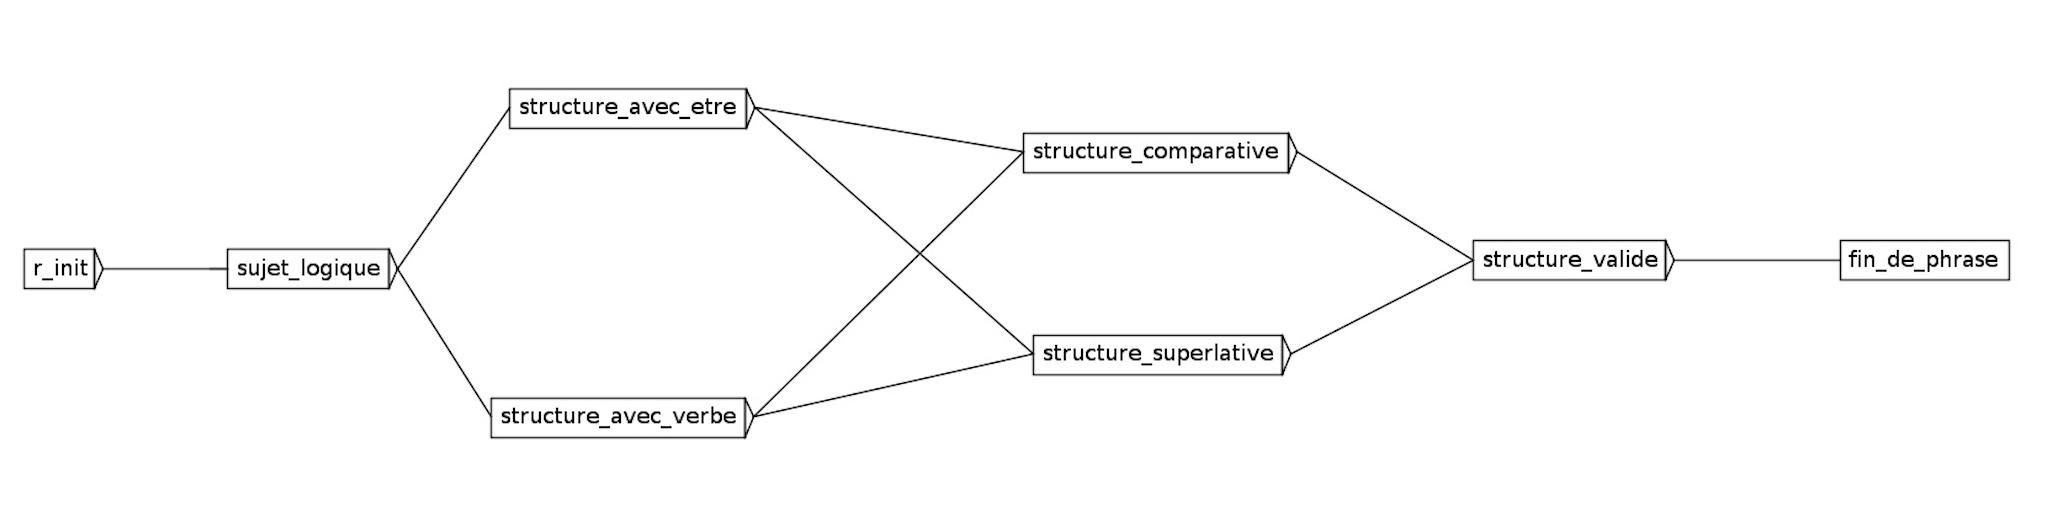
\includegraphics[width=1\linewidth]{./chap/img/dfa.png} \\

La plus grande partie du travail fut celle concernant les transitions. Elle a pris plus de 75\% du temps. \\

Puis ces derniers jours furent consacrés au nettoyage du code, et à l'écriture de ce rapport. \\

%-------------------------------------------------------------
\newpage
\section{Liste des problèmes}

Voici la liste des problèmes rencontrés. Ils sont présenter par ordre chronologique du plus ancien au plus récent. \\

{\small{
\begin{tabular}{|P{1cm}|m{7cm}|m{7cm}|}
\hline
\textbf{Num} & \textbf{Problème ou questionnement} & \textbf{Solution ou réponse} \\
\hline \hline
1 &  Sur quelle base doit-on fonder notre raisonnement ?
& Nous avons pensé que les \textbf{POS} étaient plus indiqués. Dans de rares cas, nous avons aussi utilisé le lemme. \\
\hline
2 & Comment formaliser une structure comparative ou superlative ?   
& Par l'\textbf{observation}, et en avançant pas à pas. \\
\hline
3 &  N'avons-nous pas besoin d'avoir des informations sur les mots et les phrases ?
& Si, nous nous sommes appuyé sur \textbf{treetagger}. \\
\hline
4 & Comme utiliser le même automate pour les deux langues ?
& Heureusement, le français et l'anglais ont des structures assez similaires, dans ce cas précis au moins. Il a seulement fallu prendre en compte le fait que le tagger analyse de manière plus fine en anglais. D'où l'utilité du fichier \textbf{l3\_pos.py}. \\
\hline
\end{tabular}
}}



\chapter{Résultats}
\label{sec-6}

\section{Fichiers finaux}

Les résultats du programme sont inscrits dans deux fichiers par langue : 
\begin{itemize}
    \item phrases\_*\_results.txt,
    \item phrases\_*\_analyse\_detaillee.txt\footnote{* : en ou fr}.
\end{itemize}

~\\ Le premier se présente ainsi : \\ 


\fbox{
\begin{minipage}{.85\textwidth}
\footnotesize{

\texttt{5 : Jean est le moins fort.}
 
\texttt{\hspace{.5cm} ----> OUI : Reconnaissance réussie.} 

\texttt{\hspace{1cm} Je pense que c'est une structure de comparaison. } 

%----------------------------------------------------------------------------
} 
\end{minipage} 
}

~~\\

Le seconde nous donne une analyse détaillée et se présente ainsi : \\ 

{ \Huge{PAGE SUIVANTE ---> } }

\newpage
\fbox{
\begin{minipage}{.85\textwidth}
\footnotesize{
\texttt{\hspace{.5cm} Phrase numéro 2 : The fish is smaller than The dog.} \\
  \\
\texttt{Key : 0 +++ forme : The +++ pos : DT +++ lemme : the}  \\
\texttt{Key : 1 +++ forme : fish +++ pos : NN +++ lemme : fish}  \\
\texttt{Key : 2 +++ forme : is +++ pos : VBZ +++ lemme : be}  \\
\texttt{Key : 3 +++ forme : smaller +++ pos : JJR +++ lemme : small}  \\
\texttt{Key : 4 +++ forme : than +++ pos : IN +++ lemme : than}  \\
\texttt{Key : 5 +++ forme : The +++ pos : DT +++ lemme : the}  \\
\texttt{Key : 6 +++ forme : dog +++ pos : NN +++ lemme : dog}  \\
\texttt{Key : 7 +++ forme : . +++ pos : SENT +++ lemme : .}  \\
 \\
\texttt{On est au mot 'The' de pos 'le+' } \\
\texttt{\hspace{1cm} 	Le couple a chercher est : ('r\_init', 'le+')} \\
\texttt{\hspace{1cm} 	== Nous sommes dans 'sujet\_logique' ==} \\
 \\
\texttt{On est au mot 'fish' de pos 'nom' } \\
\texttt{\hspace{1cm} 	Le couple a chercher est : ('sujet\_logique', 'nom')} \\
\texttt{\hspace{1cm} 	== Nous sommes dans 'sujet\_logique' ==} \\
 \\
\texttt{On est au mot 'is' de pos 'verbe\_etre' } \\
\texttt{\hspace{1cm} 	Le couple a chercher est : ('sujet\_logique', 'verbe\_etre')} \\
\texttt{\hspace{1cm} 	== Nous sommes au coeur d'une structure avec être.} \\
\texttt{\hspace{1cm} 	Il me faut avancer pour plus de détails. ==} \\
 \\
\texttt{On est au mot 'smaller' de pos 'adjectif\_comparatif' } \\
\texttt{\hspace{1cm} 	Le couple a chercher est : ('structure\_avec\_etre', 'adjectif\_comparatif')} \\
\texttt{\hspace{1cm} 	== On valide la 'structure\_comparative' ==} \\
 \\
\texttt{On est au mot 'than' de pos 'que+' } \\
\texttt{\hspace{1cm} 	Le couple a chercher est : ('structure\_comparative\_valide', 'que+')} \\
\texttt{\hspace{1cm} 	== Nous sommes au coeur de 'structure\_comparative' ==} \\
 \\
\texttt{On est au mot 'The' de pos 'le+' } \\
\texttt{\hspace{1cm} 	Le couple a chercher est : ('structure\_comparative', 'le+')} \\
\texttt{\hspace{1cm} 	== Nous sommes au coeur de 'structure\_comparative' ==} \\
 \\
\texttt{On est au mot 'dog' de pos 'nom' } \\
\texttt{\hspace{1cm} 	Le couple a chercher est : ('structure\_comparative', 'nom')} \\
\texttt{\hspace{1cm} 	== On valide la 'structure\_comparative' ==} \\
 \\
\texttt{On est au mot '.' de pos 'ponctuation' } \\
\texttt{\hspace{1cm} 	Le couple a chercher est : ('structure\_comparative\_valide', 'ponctuation')} \\
\texttt{\hspace{1cm} 	== Nous sommes à la fin de la phrase ==} \\
 \\
\texttt{ !!! OUI : Reconnaissance réussie.} \\
\texttt{ Je pense que c'est une structure de comparaison.} \\
%----------------------------------------------------------------------------

}
 \end{minipage}
 }

%~~\\



\chapter{Limites et ouvertures}
\label{sec-7}


 \section{Limites}

Si nous sommes un peu content du programme, nous sommes aussi conscient de ses limites. \\

Parmi les limites de notre automate  : 
\begin{itemize}
\item Il ne peut analyser que des phrases à deux membres maximum (A et B dans le cas d'une structure comparativw. A dans une phrase à structure superlative.). \\

\item Il ne peut analyser les phrases interrogatives pour le moment, surtout en anglais (ex : Is it bigger ? ). \\
 
\item Il n'est pas exhaustif. À l'échelle d'une langue, 200 phrases ou cas ne représentent pas grand chose. \\

\item Au sein même des motifs reconnus, il y a possibilité que certains puissent entrer en conflit avec d'autres. Un corpus plus grand et du temps auraient pu aider. \\

\item Enfin, comme toujours, nous aurions aimé affiner le programme, proposer plus d'options.
\end{itemize}

\section{Ouverture et réflexions diverses}

Toutes les conclusions de notre devoir du Semestre 5 s'appliquent à nouveau ici.

De plus, programmer cet automate m'a permis de me rendre compte de ce que peut être un travail linguistique (le fait de répertorier des cas, de les analyser, de modifier ou ajouter des transitions au fur et à mesure). \\

Ce fut un grand exercice d'observation voire de méditation. On pense tous savoir ce qu'est une chose (ici une comparaison). La formaliser est une autre paire de manche. J'ai passé des heures à juste essayer de comprendre comment mon cerveau analyse une phrase et en déduit si elle est ou non comparative. Ce fut clairement le plus intéressant. \\

Enfin, si nous ne devions garder qu'une phrase de cette année, ce serait \textbf{«Testez votre programme sur un corpus.»}. \\










% HK
\end{document}